\documentclass[12pt, a4paper]{article}
\usepackage{caption}
\usepackage{graphicx}
\usepackage{hyperref}
\hypersetup{
    colorlinks,
    citecolor=black,
    filecolor=black,
    linkcolor=black,
    urlcolor=black
} 

\usepackage{tikz-network}
\usepackage{amsmath, amsfonts, amssymb, amsthm}
\usepackage{algpseudocode}
\usepackage{algorithm}
\title{Computer Architecture\\and system programming}
\date{2022}
\author{Kristoffer Klokker}

\usepackage{xcolor,listings}
\usepackage{textcomp}
\usepackage{color}
\usepackage{listings}
\definecolor{codegreen}{rgb}{0,0.6,0}
\definecolor{codegray}{rgb}{0.5,0.5,0.5}
\definecolor{codepurple}{HTML}{C42043}
\definecolor{backcolour}{HTML}{F2F2F2}
\definecolor{bookColor}{cmyk}{0,0,0,0.90}  
\color{bookColor}

\lstset{upquote=true}

\lstdefinestyle{mystyle}{
    backgroundcolor=\color{backcolour},   
    commentstyle=\color{codegreen},
    keywordstyle=\color{codepurple},
    numberstyle=\numberstyle,
    stringstyle=\color{codepurple},
    basicstyle=\footnotesize\ttfamily,
    breakatwhitespace=false,
    breaklines=true,
    captionpos=b,
    keepspaces=true,
    numbers=left,
    numbersep=10pt,
    showspaces=false,
    showstringspaces=false,
    showtabs=false,
    tabsize=3,
}


\lstset{style=mystyle}
\usepackage{zref-base}

\makeatletter
\newcounter{mylstlisting}
\newcounter{mylstlines}
\lst@AddToHook{PreSet}{%
  \stepcounter{mylstlisting}%
  \ifnum\mylstlines=1\relax
    \lstset{numbers=none}
  \else
    \lstset{numbers=left}
  \fi
  \setcounter{mylstlines}{0}%
}
\lst@AddToHook{EveryPar}{%
  \stepcounter{mylstlines}%
}
\lst@AddToHook{ExitVars}{%
  \begingroup
    \zref@wrapper@immediate{%
      \zref@setcurrent{default}{\the\value{mylstlines}}%
      \zref@labelbyprops{mylstlines\the\value{mylstlisting}}{default}%
    }%
  \endgroup
}

% \mylstlines print number of lines inside listing caption
\newcommand*{\mylstlines}{%
  \zref@extractdefault{mylstlines\the\value{mylstlisting}}{default}{0}%
}
\makeatother


\newcommand\numberstyle[1]{%
    \footnotesize
    \color{codegray}%
    \ttfamily
    \ifnum#1<10 0\fi#1 |%
}


\begin{document}
	\maketitle
	\clearpage
	\tableofcontents
	\clearpage
	\section{2019}
		\subsection{Question}
			While decompiling a program you encounter the following hard-coded bytes, shown in hex-adecimal:\\
			$A=0x6d$\\
			$B=0xb3$
			\subsubsection{Convert $A$ and $B$ to binary}
				$A=0110 1101$\\
				$B=1011 0011$\\
				For the conversion each value of the hex number can be directly converted to its 4 bit equivalent.
			\subsubsection{Interpret $A$ and $B$ as signed integers in two’s complement representation. What aretheir decimal values?}
				$A=64+32+8+4+1=109$
				$B=-128+32+16+2+1=-77$
				Using the twos compliment the binary value can be converted to $A=109$ and $B=-77$
			\subsubsection{With the same interpretation of A and B as above, consider their potential multiplication using Booth’s algorithm.}

\begin{table}[h!]
\begin{tabular}{|l|l|l|l|l|l|}
B as multiplier\\
\hline
qn & q[n+1] & BR & AC & QR & sc\\
\hline
& & initial & 0000 0000  & 1011 0011  & 8\\
\hline
1 & 0 & A = A - BR &01001010 & & \\
\hline
& &  rightShift & 0010 0101  & 0101 1001  & 7\\
\hline
1 & 0 & A = A + BR & 10010010 & & \\
\hline
& &  rightShift & 1100 1001  & 0010 1100  & 6\\
\hline
0 & 0 &  rightShift & 1110 0100  & 1001 0110  & 5\\
\hline
0 & 0 &  rightShift & 1111 0010  & 0100 1011  & 4\\
\hline
1 & 0 & A = A - BR &00111100 & & \\
\hline
& &  rightShift & 0001 1110  & 0010 0101  & 3\\
\hline
1 & 0 & A = A + BR & 10001011 & & \\
\hline
& &  rightShift & 1100 0101  & 1001 0010  & 2\\
\hline
0 & 0 &  rightShift & 1110 0010  & 1100 1001  & 1\\
\hline
1 & 0 & A = A - BR &00101100 & & \\
\hline
& &  rightShift & 0001 0110  & 0110 0100  & 0\\
\hline
\end{tabular}
\end{table}

\begin{table}[h!]
\begin{tabular}{|l|l|l|l|l|l|}
A as multiplier\\
\hline
qn & q[n+1] & BR & AC & QR & sc\\
\hline
& & initial & 0000 0000  & 0110 1101  & 8\\
\hline
1 & 0 & A = A - BR &00110011 & & \\
\hline
& &  rightShift & 0001 1001  & 1011 0110  & 7\\
\hline
0 & 0 &  rightShift & 0000 1100  & 1101 1011  & 6\\
\hline
1 & 0 & A = A + BR & 10111111 & & \\
\hline
& &  rightShift & 1101 1111  & 1110 1101  & 5\\
\hline
1 & 0 & A = A - BR &00010010 & & \\
\hline
& &  rightShift & 0000 1001  & 0111 0110  & 4\\
\hline
0 & 0 &  rightShift & 0000 0100  & 1011 1011  & 3\\
\hline
1 & 0 & A = A + BR & 10110111 & & \\
\hline
& &  rightShift & 1101 1011  & 1101 1101  & 2\\
\hline
1 & 0 & A = A - BR &00001110 & & \\
\hline
& &  rightShift & 0000 0111  & 0110 1110  & 1\\
\hline
0 & 0 &  rightShift & 0000 0011  & 1011 0111  & 0\\
\hline
\end{tabular}
\end{table}
Result = 01100100
				\begin{itemize}
					\item How many rounds would be performed during the algorithm?  - 8 rounds
					\item How many additions/subtractions would be needed? - 5 operations for both ways of multiplying
				\end{itemize}
			\subsubsection{Still interpreting $A$ and $B$ as signed integers in two’s complement representation, perform the subtraction $B-A$ in binary. Indicate the result and argue whether overflow occurred or not.}
				$\overline{A}=1001 0010$\\
				$B+(\overline{A}+1)$\\
				 1011 0011\\
				 1001 0011\\
				10100 0110\\
				First the value of $A$ is negated and one is added to get the actual negated decimal value. Then the two values is added together.\\
				It can be seen that overflow does occur.\\[4mm]
			Consider the following two single-precision floating point numbers following the IEEE 754 standard:\\
			C=0 1000 0011 1011 0101 000000000000000\\
			D=0 1000 1001 0011 1010 000000000000000
			\subsubsection{What is the decimal value of $C$ and $D$?}
				C=1.
		\subsection{Question}
			In the following questions, when writing the negation of a Boolean expression you may speedup writing by using, e.g., $A'$ instead of $\overline{A}$,$(AB)'$ instead of $\overline{AB}$, and $A'B'$ instead of $\overline{A}\overline{B}$.Though, be careful with correct grouping of expressions.\\[4mm]
			Consider the following Karnaugh map for a Boolean function $F$. For some inputs there isno requirement for a specific output, indicated by $d$ (“don’t care”)\\
			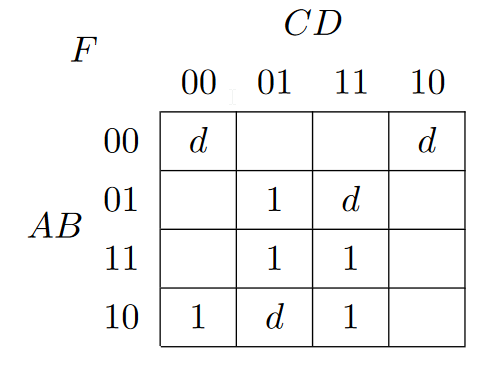
\includegraphics[width=200px]{assets/2.png}
			\subsubsection{Write the truth table for $F$}
				\begin{table}[h!]
				\begin{tabular}{|l|l|l|l|l|}
				\hline
				A&B&C&D&F\\
				\hline
				0&0&0&0&d\\
				\hline
				1&0&0&0&1\\
				\hline
				0&1&0&0&0\\
				\hline
				1&1&0&0&0\\
				\hline
				0&0&1&0&d\\
				\hline
				1&0&1&0&0\\
				\hline
				0&1&1&0&0\\
				\hline
				1&1&1&0&0\\
				\hline
				0&0&0&1&0\\
				\hline
				1&0&0&1&d\\
				\hline
				0&1&0&1&1\\
				\hline
				1&1&0&1&1\\
				\hline
				0&0&1&1&0\\
				\hline
				1&0&1&1&1\\
				\hline
				0&1&1&1&d\\
				\hline
				1&1&1&1&1\\
				\hline
				\end{tabular}
				\end{table}
				Using the Karnaugh map a truth table with the 16 possible scenarios can be written out from the four variables A,B,C, and D
			\subsubsection{Based on the Karnaugh map, write a minimal Boolean expression for $F$.}
				The karnaugh maps can be circled by two circles four sized circles around the two middle groups of ones and d's.\\
				Lastly a cicle of size two can be done around the one in the down right corner and the d next to it.\\
				This will create the expression
				$$F=AD+BD+A(BC)'$$
		\subsection{Question}
			A byte-addressable machine with 24-bit addresses has a 2-way set associative cache, where each line can hold a block of 16 bytes. At this time the cache is in the following state, wherethe tags are written in hexadecimal.\\
			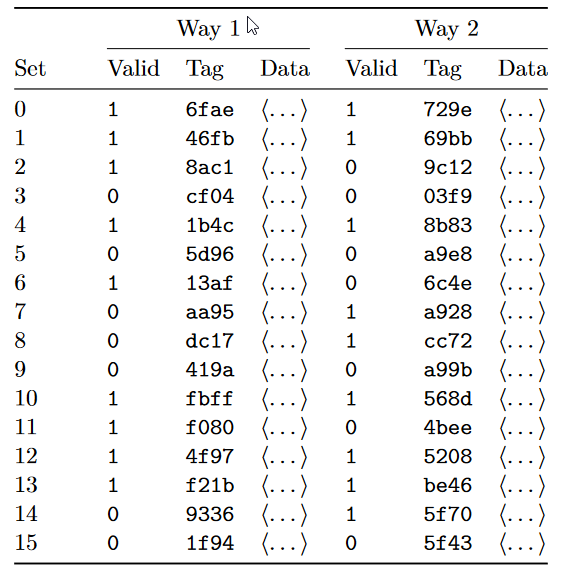
\includegraphics[width=200px]{assets/3.png}
			\subsubsection{Describe the address format for using the cache}
				Offset / Word field = log(block size) = log(16)$=4$ bit\\
				Index / Set field = log(set size)=log(16)$=4$bit\\
				Line numbers: $24$\\
				Tag = Addresse space - Offset - Index $= 24-4-4=16$
				making the address format:\\
				Tag 16 bit, Set 4 bit, Word 4 bit
			\subsubsection{Imagine 6 alternate realities where the next memory request is to read or write to each of the following addresses (written here in hexadecimal). For each scenario, describe whether there is a hit or miss in the cache.}
				\begin{enumerate}
					\item 568da3 - set: 10, tag: 568d - Hit
					\item 419a99 - set: 9, tag: 419a - Not valid
					\item 1f005d - set: 5, tag: 1f00 - Miss
					\item 69bb1b - set: 1, tag: 69bb - Hit
					\item ab61ca - set: 1, tag ab61 - Miss
					\item 1b4c4e - set: 4, tag: 1b4c - Hit
				\end{enumerate}
			\subsubsection{The cache has multiple lines per set, so the depiction above does not show all fields. Assume the replacement algorithm used in the cache is LRU, which maintains an additional bit per cache line. Compared to the actual data stored in the cache, how many percent additional memory is used in the cache for all required meta-data?}
				For LRU a bit for each line is needed.\\
				Therefore the LRU is $1 \cdot 16 =16$ bit\\
				The cache itself is 16 lines of 4 bit set, 2 times (1 bit valid, 16 bit tag) therefore $16\cdot (4+2(1+16))=608$\\
				In total the meta data is $16+608=624$ bit.\\
				The cache data is two blocks of 16 bytes pr line $16\cdot 16\cdot 2 = 512$ byte $=256\cdot 8=4096$ bit\\
				Therefore making the meta data being $\frac{624}{4096}=15.23\%$
			\subsubsection{We would like to use this cache design for the cache in each processor in an symmetric multi-processing system. However, the caches are to be kept coherent using the MESI protocol. Which changes to the cache organisation are needed, if any?}
				It can be adopted by making the validation 1 bit larger giving it the four possible combinations needed for MESI
		\subsection{Question}
			You find yourself debugging a program which sends and receives commands over the Internet. Due to the unreliability of the network connection the program uses error-correction codes for messages. Specifically, each 8-bit message is encoded as a 12-bit Hamming code
			\subsubsection{The program would like to send the following 8 bits of data, written from left to right as $d1,d2,. . . ,d8$:1111 0001. Compute the corresponding 12-bit Hamming code, and indicate the check bits.}
				The check bits is calculated as, where an odd number of ones is 1 and 0 if even\\
				$C1=D1,D2,D4,D5,D7=1,1,1,0,0=1$\\
				$C2=D1,D3,D4,D6,D7=1,1,1,0,0=1$\\
				$C4=D2,D3,D4,D8=1,1,1,1=0$\\
				$C8=D5,D6,D7,D8=0,0,0,1=1$\\
				Making the whole data bit:\\
				C1,C2,D1,C4,D2,D3,D4,C8,D5,D6,D7,D8\\
				1 1 1 0 1 1 1 1 0 0 0 1
			\subsubsection{The program is receives the following 12 bits in response, written from left to right as $b1,b2,. . ., b12$ :1001 1100 0001. Assuming that at most 1 single-bit error has occurred,compute the 8-bit message.}
				C1,C2,D1,C4,D2,D3,D4,C8,D5,D6,D7,D8
				1   0   0   1   1    1   0   0   0   0   0   1
				Calculating the check bits\\
				$C1=D1,D2,D4,D5,D7=0,1,0,0,0=1$ Match\\
				$C2=D1,D3,D4,D6,D7=0,1,0,0,0=0$ Wrong\\
				$C4=D2,D3,D4,D8=1,1,0,1=1$ Match\\
				$C8=D5,D6,D7,D8=0,0,0,1=0$ Wrong\\
				Since the C2 and C8 share D6 it must be flipped making the original message:\\
				0110 0101 
	\section{2018}
		\subsection{Question}
			Consider the two 5 bit pattersn $s=$10011 and $T=$01010.
			\subsubsection{ Interpret $S$ and $T$ as unsigned integers. What are their decimal values?}
				$S=2^5+2^1+2^0=19$\\
				$T=2^4+2^1=10$\\
			\subsubsection{Interpret $S$ and $T$ as signed integers in two’s complement representation. What are their decimal values?}
				$S=-2^5+2^1+2^0=-13$\\
				$T=2^4+2^1=10$\\
				The first bit will then be used as a negative value when calculated, and since the first value is already zero in $T$ the value does not change.
			\subsubsection{Interpret $S$ and $T$ as signed integers in two’s complement representation. Multiply $S$ and $T$ using Booth’s algorithm. Show}
				\begin{itemize}
					\item The intial state of the algorithm
					\item For eeach step the actions taken the resulting state
					\item The final produkt in twos complement representation and its decimal value
				\end{itemize}
				\begin{table}[h!]
				\begin{tabular}{|l|l|l|l|l|l|}
				multiplicand: 10011 & Multiplier: 01010 \\
				\hline
				Q[0] & Q-1 & Log & A & Q & SC\\
				\hline
				0 & 0 & initial & 0 0000  & 0 1010  & 5\\
				\hline
				0 & 0 &  rightShift & 0 0000  & 0 0101  & 4\\
				\hline
				1 & 0 & A = A - M &0 1101  & 0 0101 &\\
				\hline
				& &  rightShift & 0 0110  & 1 0010  & 3\\
				\hline
				0 & 1 & A = A + M & 1 1001  & 1 0010 &\\
				\hline
				& &  rightShift & 1 1100  & 1 1001  & 2\\
				\hline
				1 & 0 & A = A - M &0 1001  & 1 1001 &\\
				\hline
				& &  rightShift & 0 0100  & 1 1100  & 1\\
				\hline
				0 & 1 & A = A + M & 1 0111  & 1 1100 &\\
				\hline
				& &  rightShift & 1 1011  & 1 1110  & 0\\
				\hline
				\end{tabular}
				\end{table}
				\begin{table}[h!]
				\begin{tabular}{|l|l|l|l|l|l|}
				multiplicand: 01010 & Multiplier: 10011 \\
				\hline
				Q[0] & Q-1 & Log & A & Q & SC\\
				\hline
				1 & 0 & initial & 0 0000  & 1 0011  & 5\\
				\hline
				1 & 0 & A = A - M &1 0110  & 1 0011 &\\
				\hline
				& &  rightShift & 1 1011  & 0 1001  & 4\\
				\hline
				1 & 1 &  rightShift & 1 1101  & 1 0100  & 3\\
				\hline
				0 & 1 & A = A + M & 0 0111  & 1 0100 &\\
				\hline
				& &  rightShift & 0 0011  & 1 1010  & 2\\
				\hline
				0 & 0 &  rightShift & 0 0001  & 1 1101  & 1\\
				\hline
				1 & 0 & A = A - M &1 0111  & 1 1101 &\\
				\hline
				& &  rightShift & 1 1011  & 1 1110  & 0\\
				\hline
				\end{tabular}
				\end{table}
				Result = 1101111110=$-2^9+2^8+2^6+2^5+2^4+2^3+2^2+2^1=-130$\\[4mm]
				Consider 9-bit signed integers in two’s complement representation
			\subsubsection{What is the range of integers are representable in this format?}
				The lowest value is $-2^8=-256$ where the most significant bit is 1 and the rest is zero. The highest will be everything is one except the most significant bit $2^7+2^6+2^5+2^4+2^3+2^2+2^1+2^0=255$
			\subsubsection{ Which bit pattern represents the lowest and highest representable values?}
				Highest: 10000000\\
				Lowest: 01111111\\[4mm]
			Consider the following two single-precision floating point numbers following the IEEE 754 standard:\\
			$A$= 0 0111 0001 0011 0100 000000000000000\\
			$B$= 0 0111 0011 1001 1000 000000000000000
			\subsubsection{Give the decimal value of $A$ and $B$ in the normalised form $S\cdot 2^E$ where $1\leq S \leq 2$}
				$A$\\
				Sign: +\\
				Power: 11100010 - 127 = 99\\
				Decimal: 1.01101000000000 = 1.40625\\
				$1.40625\cdot 2^{99}$\\
				$B$\\
				Sign: +\\
				Power: 01110011 - 127 = -12\\
				Decimal: 110011000000000 = 1.59375\\
				$1.59375\cdot 2^{-12}$
			\subsubsection{Perform the addition of $A$ and $B$ in binary arithmetic}
				For the calculation the zeroes is described as (number of zeroes)x0 instead of writing them out.\\
				X exponent:  99\\
				Y exponent:  -12\\
				X fraction:  10110100000000000000000\\
				Y fraction:  110011000000000000000000\\
				First align mantisse\\
				Add 111 zeroes to Y to align\\
				Y fraction: (111)x0  110011000000000000000000
				Adding X fraction and Y fraction\\
				101101 (128)x0 110011000000000000000000\\
				Sum:  101101 (105)x0 110011000000000000000000\\
				Convert sum back into IEEE 754 format, by removing the first 1 if the sum and using the largest exponent\\
				0 11100010 01101000000000000000000
		\subsection{Question}
			In the following questions, when writing the negation of a Boolean expression you may speedup writing by using, e.g., $A'$ instead of $\overline{A}$,$(AB)'$ instead of $\overline{AB}$, and $A'B'$ instead of $\overline{A}\overline{B}$.Though, be careful with correct grouping of expressions.\\[4mm]
			Consider the following truth table for a Boolean function that we would like to implementin hardware with the smallest circuit we can reasonably find. This means that we should take advantage of the fact that for some inputs there are no requirement for a specific output,indicated by $d$ (“don’t care”).\\
			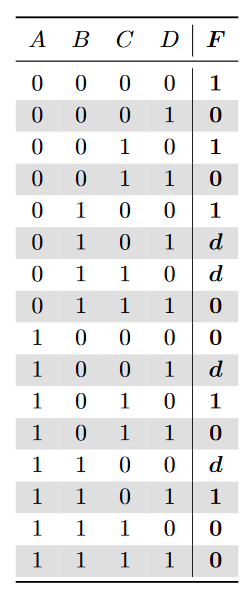
\includegraphics{assets/183.png}
			\subsubsection{As a first solution, write a Boolean expression for $F$ in sum-of-products form.}
				$F=(ABCD)'+C(ABD)'+B(ACD)'+AC(DB)'+ABCD'$
			\subsubsection{Draw the Karnaugh map for $F$}
				\begin{table}[h!]
				\begin{tabular}{l|l|l|l|l|l|l|}
					&&&CD&&\\
					\hline
					&&00&01&11&10\\
					\hline
					&00&1&&&1\\
					\hline
					AB&01&1&d&&d\\
					\hline
					&11&d&1&&\\
					\hline
					&10&&d&&1\\
					\hline
				\end{tabular}
				\end{table}
			\subsubsection{ Based on the Karnaugh map, write a minimal Boolean expression for $F$.}
				$F=(AD)'+BC'+C(BD)'$
		\subsection{Question}
			We are tasked with designing a new cache for a machine with 32-bit addresses, where the addressable unit is a single 8-bit byte. The size of each cache line must be able to hold 64 bytes of data, and in total the cache must be of size 128 KiB (where 1KiB is 1024B). First we consider implementing the cache with direct mapping\\
			\subsubsection{How many lines will the cache have?}
				Physical address bits = $32$ bit\\
				Block size = 64 bytes = $2^6$B\\
				Cache size = $128\cdot 1024=2^{17}$B\\
				Number of lines = Cache size/Block size= $2^{11}$
			\subsubsection{Describe the address format for the cache?}
				Block offset = log(Block size) = 6 bits\\
				Line offset = log(Number of lines) = 11 bits\\
				Tag size = 32-6-11=15 bits\\
				Making the address format: Tag 15 bits | Line offset 11 bits | Block offset 6 bits
			\subsubsection{Besides the actual data, for each line we must also store a tag and a valid-bit. Compared to the memory used for data, how many percent additional memory do we need for the required meta-data?}
				The tag was found to be 15 bits and a valid bit making the meta data 16 bit pr. line.\\
				This making the meta data take up $\frac{16b}{64\cdot 8b}=3.12\%$ of the stored data.\\[4mm]
			Alternatively we now consider an implementation as a 8-way set associative cache
			\subsubsection{How many sets will the cache have?}
				The number of sets will be = number of lines/8=$2^3$
			\subsubsection{Describe the address format for the cache?}
				The block offset is still 6 bits\\
				The set offset will be = log(number of sets)=3 bits\\
				Making the tag = 32-6-3=23 bits
			\subsubsection{Besides the actual data, for each line we must also store a tag and a valid-bit. Compared to the memory used for data, how many percent additional memory do we need for therequired meta-data?}
				The tag is now 23 bits so the meta data is 24 bits.\\
				This making the meta data take up $\frac{24b}{64\cdot 8b}=4.69\%$ of the stored data.\\[4mm]
			The two cache designs are now compared on the effect on memory access times.
			\subsubsection{The direct-mapped cache has an access time for each memory request of 4ns and a miss rate of $5\%$. After a miss the request goes to main memory, which adds 103ns to the access time (including the subsequent cache update). What is the average access time?}
				$4ns\cdot 0.95+103ns\cdot 0.05=8.95ns$
			\subsubsection{Due to its increased complexity the set-associative cache has a slightly higher accesstime of 6ns, though the miss rate drops to just $3\%$. As the cache update in case of a miss is also slightly slower, the added access time is now 104ns. What is the averageaccess time for this setup?}
				$6ns \cdot 0.97+104ns\cdot 0.03=8.94$
		\subsection{Question}
			Consider a symmetric multi-processing system with two processors $P1$ and $P2$. They each have their own cache which are kept coherent using the MESI protocol. For this question we look at two blocks of memory $b1$ and $b2$ where we assume they are mapped to the caches such that they can be present simultaneously. Initially (at time $t0$), the state of $b1$ is “invalid” in the cache of both $P1$ and $P2$, while the state of $b2$ is “exclusive” in $P1$ and “invalid” in $P2$.
			\subsubsection{For the following sequence of events, show the resulting MESI state of each block ineach processor.}
				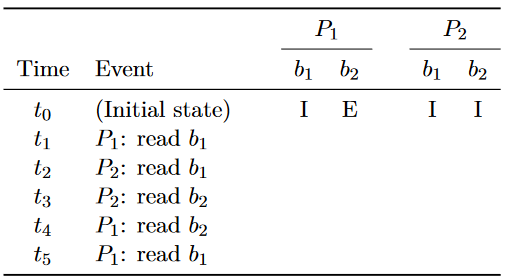
\includegraphics[width=300px]{assets/184.png}\\
				$t1$ - Read b1 from memory and sets it as exclusive\\
				$t2$ - Read b1 from memory and set as shared and notifies p1 to set b1 as shared\\
				$t3$ - Read b2 from memory and set as shared and notifies p1 to set b2 as shared\\
				$t4$ - Nothing changes\\
				$t5$ - Nothing changes
		\subsection{Question}
			Assume the following content in the main memory(all numbers are in hexadecimal format with omitted leading zeros):\\
			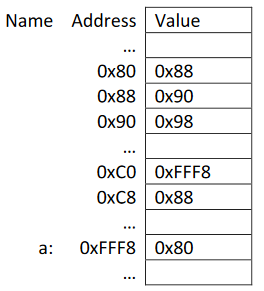
\includegraphics[width=200px]{assets/164.png}\\
			During the course of your program, you have defined the local variables a and b on the stack as follows:
			\begin{lstlisting}
...
long **a
...\end{lstlisting}
			Assume  you  are  working  on  a  64 Bit  Linux  machine  using  the  gcc;thus long  values  as  well  as addresses  consume  64  bit.The  execution  of  your  program  has  led  to  the  memory  content  as displayed above.
			\subsubsection{To what values do the following expressions evaluate}
				\begin{itemize}
					\item **a - 0x80
					\item \&a - 0xFFF8
					\item **(a+1) - 0xFFF0
				\end{itemize}
			\subsubsection{What is a void pointerand what is such a pointer used for?}
				A void pointer is a pointer which points to any data type.\\
				A void pointer can be used as a generic pointer.
			\subsubsection{Declare  a function  pointer “ptr” to  a  function  requiring two  integersas  arguments returning a pointerto a long variable.}
				\begin{lstlisting}
long func(int a, int b);

long (*ptr)(int,int) = \&func\end{lstlisting}
			Now consider the following C function calculating the scalar product of two vectors a and  b of dimension d. The program is written for a 32 Bit Linux machine.
				\begin{lstlisting}
int scalarproduct(int* a, int* b, int d)
{
	int ret = 0;
	int i;
	for(i = 0; i < d; i++){
		ret += a[i]*b[i];
	}
	return ret;
}\end{lstlisting}
			\subsubsection{Give  the stack-framerelevant for the function relative to the function’s stack base pointer (\%ebp).   Identify   all   variables   and   parameters   of   the   C-Function.   Use   the following table as template (produce a table similar to this one):}
				\begin{table}[h!]
\begin{tabular}{|l|l|}
\hline
\textbf{Location in stack} & \textbf{Contant}   \\ \hline
...                        &                    \\ \hline
-8(\%ebp)                  & Loval variable     \\ \hline
-4(\%ebp)                  & Local variable     \\ \hline
(\%ebp)                    & Old base pointer   \\ \hline
4(\%ebp)                   & Return address     \\ \hline
8(\%ebp)                   & function arguments \\ \hline
...                        &                    \\ \hline
\end{tabular}
\end{table}
			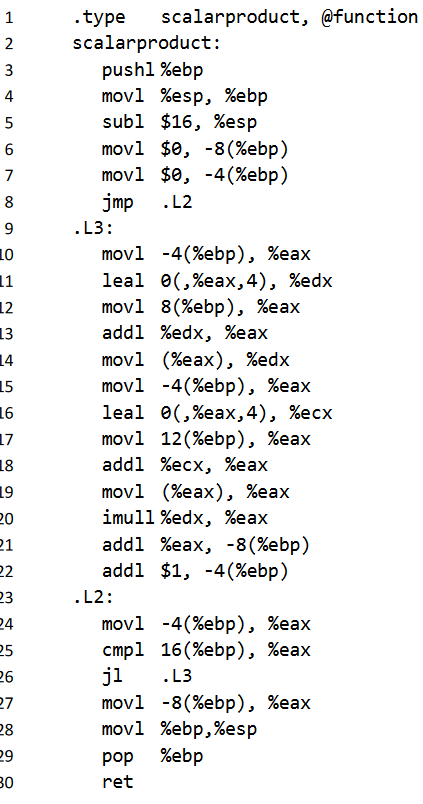
\includegraphics[width=200px]{assets/164a.png}
			\subsubsection{Identify the lines in the assembly code where the abort condition $i < d$ is checked and where does the code continue in case the condition does not hold and where in case it does not.}
				The comparison is done at line 25, and if less jump to l3 otherwise it continues to line 27.
			\subsubsection{Identify in which lines in the assembler code the address of $a[i]$ is calculated and in which register is the value of $a[i]$ temporarily stored.}
				$a[i]$ is calculated at line 13 where first the address of a is found and then the value of i is added together.\\
				The result is then stored in \%edx
			\subsubsection{Consider line 16 in the assembly code}
				\begin{itemize}
					\item What does this line do? - The line takes the address of eax multiplies it by 4 and puts it into \%ecx
					\item Replace this line by standard arithmetid or logical operation - imull $4, (\%eax); movl (\%eax), \%ecx$
				\end{itemize}
			\subsubsection{Through which register is the result returned to the caller?}
				Througout the program the value is stored in $-8(\%ebp)$ and then moved into \%eax at line 27 and returned
				
			
\end{document}